% -- Encoding UTF-8 without BOM
% -- XeLaTeX => PDF (BIBER)

\documentclass[espanol]{cv-style}     % Add 'print' as an option into the square bracket to remove colours from this template for printing. 
                                      % Add 'espanol' as an option into the square bracket to change the date format of the Last Updated Text
%\setdefaultlanguage{spanish}
%\sethyphenation[variant=spanish]{}{}  % Add words between the {} to avoid them to be cut 

\usepackage{graphicx}

\begin{document}

\header{Salvador }{Jiménez}
\lastupdated

%----------------------------------------------------------------------------------------
% SIDEBAR SECTION  -- In the aside, each new line forces a line break
%----------------------------------------------------------------------------------------
\begin{aside}
\section{\_}
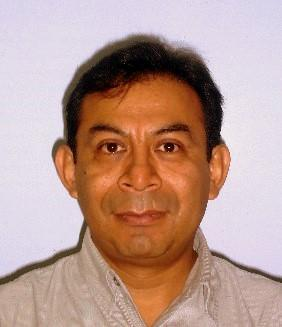
\includegraphics[width=4cm]{SJS_2007.jpg}
%
\section{Education}
\href{https://tec.mx/en}{\bf ITESM, Tec de Monterrey}
B.Sc. in Electronic Systems
Ing. Sistemas Electrónicos ISE
May 1987 
%
\section{Personal info.}
56, Mexican
NAFTA TN Visa eligibility
~
Github:// \href{https://github.com/salvador-jmz}{\bf salvador-jmz} 
LinkedIn:// \href{https://www.linkedin.com/in/salvadorjmz}{\bf salvadorjmz} 
Twitter:// \href{https://twitter.com/sjimenez}{\bf @sjimenez} 
Quora:// \href{https://www.quora.com/Salvador-Jmz}{\bf Salvador-Jmz}
%
\section{Contact}
(+52) 55 5402 5951
~
\href{mailto:sjimenez@exatec.itesm.mx}{\bf sjimenez@exatec.itesm.mx}
~
Mexico City, MX
%
\section{Languages}
Spanish (native),
English (professional working proficiency)
%
\section{Skills}
{\color{red} $\varheartsuit$} Project Management
BID/Tendering Gov. proposals
Enterprise WAN/LAN Deploymnent
NOC Design and Implementation
%
\section{Software Tools}
{\color{red} $\varheartsuit$}{\bf OpenSource} RedHat/Ubuntu/Debian Linux, PostgreSQL DataBase, LaTeX
{\bf Enterprise}
Oracle RAC, Microfocus Network Monitoring Software, RHEL, CiscoWorks LMS, Visio, MS-Project
%
\end{aside}
%----------------------------------------------------------------------------------------
% RESUME SECTION
%----------------------------------------------------------------------------------------
\vspace{0.2cm}
\section{Career Objective}
  \vspace{-0.2cm}
A self-motivated and an inspired team player, who is looking for greater opportunities of innovation and professional growth.
Inclined and experimenting on new areas like Cloud Computing, DevOps, IoT, AI and Big Data Analytics.
%----------------------------------------------------------------------------------------
% WORK EXPERIENCE SECTION
%----------------------------------------------------------------------------------------
\section{Experience}
  \vspace{-0.2cm}
\begin{entrylist}
%------------------------------------------------
\entry
  {\scalebox{.8}[1.0]{2014 - Present}}
  {\href{https://www.thalesgroup.com/es/americas/thales-mexico}{Thales Group}}
  {Mexico City, MX}
  {\jobtitle{Sr. BID/Tendering Technical Manager}\\
\textbf{*} Ensure timely responses to customer enquiries, prepare clarifications and deviations to tenders, as well as technical annexes and contract schedules.\\
\textbf{*} Take the full responsibility for the technical solution during the Sales phase.\\
\textbf{*} Understanding of the market, customer business cases and sales perspective in general; Track of the local rules and legislation.\\
\textbf{*} Be the liason between the Local Sales organization and France Engineering for general technical matters and pursuit  technical approval for BIDs greater than \$ 3M USD.\\
\textbf{*} Working with Sales local team or customer prospects to ascertain opportunities or information enquirers necessary to produce Sales proposals including technical product selection, quotation documents (BoMs), technical specifications and Statements of Work (SOW) for subcontractors.
}
%------------------------------------------ ------
\vspace{-0.3cm}
\entry
  {\scalebox{.8}[1.0]{2009--2014}}
  {Thales Group}
  {Mexico City, MX}
  {\jobtitle{NOC Work Package}\\
Design \& Implementation of the Network Operation Center for monitoring a  Video-Surveillance City Network (Mexico "Ciudad Segura")
using HP-OpenView (Microfocus) software applications:
  \begin{itemize}
    \item HP Network Node Manager (HP-NNM) \& HP SiteScope \& HP-BSM
\item HP Operations Manager \& HP Performance Insight \& HP Service Desk\\
  \end{itemize}
  }
%------------------------------------------------
%------------------------------------------------
\vspace{-0.3cm}
\entry
  {\scalebox{.8}[1.0]{2009--2009}}
  {Schweitzer Engineering Laboratories}
  {Luverne, ND}
  {\jobtitle{Electrical/Electronic Specialist}\\
As a Freelance Engineer for SEL, I supervised and coordinated the installation, wiring, interconnection and configuration of several S.E.L. Relays control
panels in a Wind-Farm Sub-station located at Luverne,ND. My team accomplished the task according Otter Tail Power Co. deadline. Acceptance Test Procedure was agreed with great customer satisfaction. Contact: Wayne Preston wpreston@otpco.com \\
  }
%------------------------------------------------
%------------------------------------------------
\entry
  {\scalebox{.8}[1.0]{2003 - 2009}}
  {MVSnet}
  {Mexico City, MX}
  {\jobtitle{IT Manager}\\
\textbf{*} Responsible to manage the I.T. infrastructure for a WISP (WiMaX Internet Service Provider)
}
%------------------------------------------------
\entry
  {\scalebox{.8}[1.0]{1987 - 2003}}
  {Banpais $\rightarrow$ Mifel $\rightarrow$ Gasoplus}
  {Mexico City, MX}
  {\jobtitle{Support Engineer $\rightarrow$ IT Manager}\\
\textbf{*} From Maintenance \& support activities to Telecomm. Manager in a National Bank.
}
\end{entrylist}
%-----------------------------------------------------
%------------------------------------------------
% EDUCATION SECTION
%----------------------------------------------------------------------------------------
\vspace{-0.2cm}
\section{Professional Training}
\vspace{-0.2cm}
\begin{tabular}{ p{5em} p{6em} p{20em} rp{6em}}
2019 & Online & Cybersecurity Fundamentals & Thales University\\
2016 & Online & Passport to System Engineering & Thales University\\
2014 & Online & System Architecting & Thales University\\
2011 & Paris, FR & HP NNMi now Microfocus & Axel-IT\\
2008 & Tokyo, JP & WiMAX BST Functionality Tests & NEC\\
2007 & MN, USA & NextNet Expedience WiMAX System & NextNet Wireless\\
1995 & MD, USA & VSAT Satellite System & Hughes Network Sys.\\
% 1994 & Mex. DF & Configuración Enrutadores Cisco & Red-Uno\\
\end{tabular}
%------------------------------------------------
%\end{entrylist}
%----------------------------------------------------------------------------------------
% AWARDS SECTION
%----------------------------------------------------------------------------------------
%\section{extracurricular}
%  \vspace{-0.2cm}
%\begin{entrylist}
%------------------------------------------------
%\entry
%{\scalebox{.8}[1.0]{2007--2008}}
%{Olimpíadas Matemáticas Argentinas}
%{}
%{Alumno aprobado en el Certamen Nacional de las 24º y %25º Olimpíadas Matemáticas Argentinas}
%------------------------------------------------
%\end{entrylist}
%  \vspace{-0.2cm}
%----------------------------------------------------------------------------------------
% INTERESTS SECTION
%----------------------------------------------------------------------------------------3
%\section{intereses}
%vspace{-0.2cm}
%\textbf{Back-end.} Sectores de análisis de datos y %categorización (Natural Language Processing, Machine %Learning); optimización de procesos; mantenimiento de %servidores y bases de datos; seguridad informática.
%----------------------------------------------------------------------------------------
\end{document}